\documentclass[11pt,twoside,a4paper]{article}
\usepackage[english]{babel}
\usepackage{amsmath}
\usepackage{amsthm}
\usepackage{amssymb}

\usepackage[pdfstartview=FitH,pdfpagemode=UseNone]{hyperref}
\usepackage[letterspace=40]{microtype}

\usepackage{a4wide,times}
\usepackage{graphicx}
\usepackage{color}
\usepackage[section]{placeins}

\urlstyle{same}
\linespread{1.1}

\title{
  Emergent Architecture Design Document\\
  DuoDrive
}
\author{
    Pim van den Bogaerdt, pvandenbogaerd, 4215516\\
    Ramin Erfani, rsafarpourerfa, 4205502\\
    Robert Luijendijk, rluijendijk, 4161467\\
    Mourad el Maouchi, melmaouchi, 4204379\\
    Kevin van Nes, kjmvannes, 4020871
}

\begin{document}

\maketitle
\begin{center}
TI2805 Contextproject, 2013/2014, TU Delft\\
Group 5, Computer Games\\
Version 4 (draft)
\end{center}
\clearpage


\section*{Abstract}
This document describes the architecture of the system of which our product consists. Firstly, we will describe the design goals for our final product. After that, our Software Architecture Views will be treated. Finally, a glossary can be found at the end of the document. This document will be edited and changed throughout the duration of the project to fit our current system architecture.


\clearpage
\tableofcontents

\clearpage


\section{Introduction}
In this document we will describe the architecture of the system that we will be creating during the Computer Games Contextproject. The architecture will be expanded on in a high-level form, after which the sub-components and sub-systems will be explained. This will give more insight in what the system is composed of and how the several elements of the system work together. 


\subsection{Design goals}
We will maintain four design goals throughout the duration of the project:

\begin{description}
\item[Availability] \hfill \\
    During this project our product will be \emph{continuously integrated} with the goal of having a working product running at any time. This allows us and the client to test and work with the product at any time, even before the final release.
After the final release we will want to make sure that the server is up as much as possible, especially during the time that people are visiting our client's company or area. 
\item[Replayability] \hfill \\
    A design goal that we consider to be specific for our product is replayability. We want the players to enjoy the game in such a way that the game will be replayable in both the short and long term. We want the players to find our product memorable, so they may even look forward to playing the game the next time. To reach this goal, the game should make a solid first impression, after which elements such as randomness and other unpredictable events will keep the game interesting to play.
\item[Usability] \hfill \\
    The game is designed in such a way that without, or with few, instructions the player will be able to play the game. After a few minutes, or even seconds, the player will have learned how the game mechanics work and how to play the game. The physics in the game are set to make the user experience better and giving the best possible experience to the player. \\
        The player will also be able to see his progress and see how well he is playing the game.
\item[Performance] \hfill \\
    The system will have a central server which is situated in the same room/building/area as the players who are playing the game. Also, all the players should be connected to the same network as the server is connected to. Since the server will be the machine sending and receiving the data from and to the players, it is necessary that the connection between the player and the server is fast enough. This is necessary to ensure that players will not encounter any \emph{latency issues}. \\
    In a future release we might implement a system where some of the server's calculations will be calculated locally on the player's device. This will take load off the server and may improve the connection speed throughout the game, although for now the implementation of these kinds of features are not planned yet.
    
\end{description}

\newpage

\section{Software Architecture Views}
This chapter will discuss the architecture of the system and how it is decomposed. In the first paragraph the subsystems will be decomposed and we will give an explanation about each subsystem. In the second paragraph we will elaborate upon the relations and mapping between hardware and software. Finally, in the last paragraph the data management will be explained.


\subsection{Subsystem Decomposition}
The software architecture of the system consists of three different subsystems: the server, the system for the steering player and the system for the player who controls the throttle. These different subsystems are explained in this section.

\begin{itemize}
\item Server \hfill \\
    The server is a subsystem that maintains the data flow. For example, it will send the data of the positions of the cars to all players, so that every player has a near real-time experience, where they can see other players' positions. All data sent by a player will first be sent to the server, which distributes it to the other players. There is no player-to-player data flow at this moment.
\item Steering player system \hfill \\
    The system for the steering player will only contain the view that the steering player sees. This will be a limited view, as the steering player will only see a small area in front of his car. The steering player will also not be able to throttle. 
\item Throttler system \hfill \\
    In the throttler system the ability to perform certain actions is also limited. The player will only be able to control the throttle, i.e. accelerating forward or backward and hitting the brake. By limiting the view and the possible actions, communication between the throttling player and steering player will be enforced.
\end{itemize}


\subsection{Hardware/Software Mapping}
The hardware that is used is varied in terms of the player-held device. This is because players can use any device that has Android as its operating system. The only other piece of hardware that will be required is a central computer that will serve as a central server. \\
Whereas the hardware can differ, the software that runs on it differs in three possible ways. This means that the software can run as a server, as a throttling player or as a steering player. Depending on the role, the shown user interface will be different. The server has a simplistic interface which will make it possible to start or end the server.
The mapping of the hardware and software can easily be concretised in a small diagram, which is shown on the next page:
\begin{figure}
	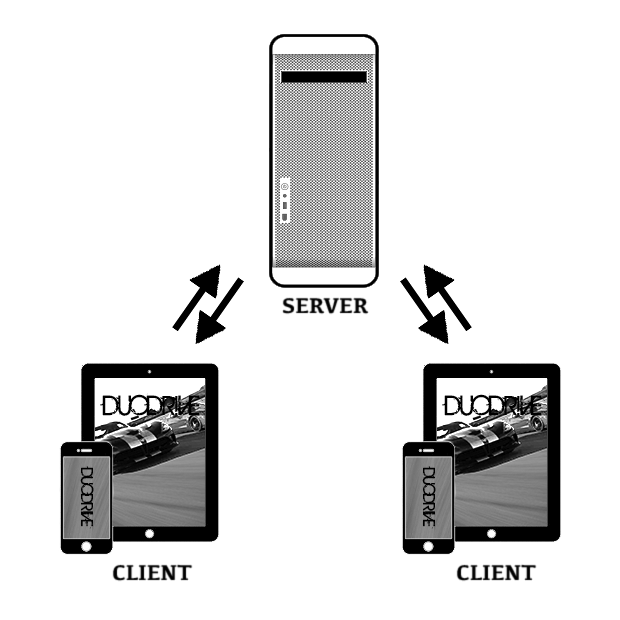
\includegraphics[width=\textwidth]{ClientServer.png}
	\caption{Hardware/Software mapping}
\end{figure}

\newpage

\subsection{Persistent Data Management}
There is no need for persistent data management in our product. There is no data that needs to be saved persistently.

\subsection{Concurrency}
Concurrency is an important aspect to take into account when dealing with a multiplayer game. Especially if this multiplayer game is one where people interact with each other in real-time.\\
Concurrency is handled in one specific way in our game, which is by using \emph{Remote Procedure Calls} (RPC).\\
\newline
Initially, we wanted to use state synchronization for sending the car position and rotation between players. State synchronization is a feature of Unity that (among other features) allows  for unreliable synchronization of the state of a GameObject (Unity Manual, 2014).\\
In our case, the state we would want to send is the position and rotation of a car. We believe this would be the preferred way of sending this data between players. However, we did not manage to have two players each update a part of the state, which would be required, because the throttler only updates the position, whereas the driver only updates the rotation.\\
\newline
Using RPC has some advantages, but it also has some drawbacks.\\
The main advantages are that RPC is easily used within Unity and that RPC allows us not to have to deal with coding the remote interactions.\\
An advantage that is specific when using RPC in Unity is that Unity itself handles the threading of RPCs. As a result of this, we did not have to worry about creating concurrency problems with our own code.\\
However, the drawbacks are that RPC waits for a server to process the call before allowing the client to continue. This means that we had to be sparse in using RPC throughout our code, for if we did not do this, the server might get congested with calls and this would influence the output of the game.\\

\newpage

\section{Classes}
\subsection{Introduction}
At the start of the project we created a class diagram to be able to get a quick view of the system as a whole and also to provide this quick view to people outside our project group. However, during the development of the project, we came to the conclusion that updating our class diagram would quickly become too messy. Unity makes use of \emph{GameObjects}, which have scripts attached to them as components. The interaction of these scripts with other scripts, classes and GameObjects depends on different variables of the GameObjects. This made it very hard for us to create and maintain a class diagram for a clear overview, even at a high level.
Instead of a class diagram, we have chosen to dedicate a section of this report to the setup of the classes and the interaction between them. This allows us to still be able to discuss the hierarchy of the classes and their interactions.

\subsection{Classes}
Within the whole project we count 43 classes, excluding test classes. Every class has been created in such a way that it has its own functionality. Where necessary or useful, we applied Design Patterns. In this project we have made use of the Strategy Pattern and Singleton Pattern. The Strategy Pattern can be seen in the setup of the  Player and Role classes. The Singleton Pattern is used in the TimeController class. Furthermore, a client-server architecture has been used since this was ideal to distribute different tasks over the server and clients. What is meant by this is that the server handles most back-end tasks, so that the smartphones/tablets, the clients, are less burdened.

\subsection{Packages}
The classes have been split into different packages. Every package has its own responsibility. In the upcoming descriptions every package and its responsibilities will been expanded on. Furthermore, if a Design Pattern has been used within a package this will also be mentioned below.

\begin{description}
\item[Behaviours] \hfill \\
    In this package we have added all classes that are attached to GameObjects as behaviours. An example of such a class is the Car class, which has the CarBehaviour-script attached to it. This script manages how the Car should behave during the game. The other Behaviour-classes are meant to manage the racing track.
\item[Cars] \hfill \\
    The Cars package contains classes which create the cars and the players attached to them. We used the Strategy Pattern to set up these classes. This was recommended to us during a meeting with mr. Bacchelli and TA Bastiaan Reijm and in practice this turned out to be much better than simply using inheritance. This is because the composition that comes with the Strategy Pattern allows for better decoupling between the player and the roles.
    \newpage
\item[Controllers] \hfill \\
    The Controller classes are all classes that, as their names suggest, control a part of the code in some way. The classes in this package are the NetworkController, TimeController and CountdownController. The first one handles all kinds of tasks associated with the network flow. The latter two control the countdown before the race starts and the timer that is shown to the players during the race.
\item[GraphicalUI] \hfill \\
    For the Graphical User Interface (GUI) of DuoDrive we have designed the following. There are several classes that implement GraphicalUIPart and draw using the Unity GUI class. A GraphicalUIConfiguration contains a list of such parts. Finally, a controller (GraphicalUIController) has a stack of configurations and draws only the top configuration of the stack.
\newline\newline
The configurations we use are predefined and added to the controller class. We have distinguished between parts and configurations so that certain parts (e.g. for the restart button) can be shared between configurations (e.g. for the driver's and throttler's GUI).
\newline\newline
We found this design helpful, because it is easy to add ("push") a new configuration to show it, and remove ("pop") it when it should not be shown. For example, the tutorial is implemented by pushing its configuration when the tutorial button is clicked. Subsequently, the configuration is popped when the tutorial is over, so that the previous GUI configuration is visible again.
\item[Interfaces] \hfill \\
    Within this package all interfaces are placed together. Some of these interfaces are not needed for the actual game, but to be able to test several classes we needed to mock them. In C\#, the programming language we chose to program in, mock-objects can only be made from virtual objects and/or interfaces. 
\item[Main] \hfill \\
    In the Main package we have two classes, Game and MainScript. Game handles the adding of cars into the game. Furthermore, the MainScript class is responsible for most of the initialization of the game. The first steps are initializing the Server, Client and Tutorial GameObjects and initializing the cars.
\item[NetworkManager] \hfill \\
    Within the NetworkManager package two classes can be found: Server and Client. The Server class handles all the operations and commands that should go to and/or through the server. The Client class handles the job that should be assigned to the newly connected player, who is in fact a new client.
\item[Utilities] \hfill \\
    The Utilities package contains some simple utility classes which are intended to access several functions with ease and without the need of the special MonoBehaviour class in Unity.
    \newpage
\item[Wrappers] \hfill \\
    In this package several wrappers are stored. These wrappers are needed so that the classes which use the interfaces as variables, will still have their functionality. However, for the input a wrapper was also made, so that we could simulate certain inputs. Without the wrapper it was impossible to test e.g. touch events and thus some methods could not be tested without them.
    
\end{description}

\subsection{Test Classes and Testing}
For this project we used Unity as our main development tool. Although we have written tests that cover a large part of the code (except for the GUI, which is intended), we do not have the tools to measure the code coverage exactly.\\
\newline
To test the server-side communication and -interaction we have made use of mocking. This has been done with the Moq-asset, which we retrieved from the Unity Asset Store.\\
\newline
To be able to mock certain classes, several interfaces had to be created. By using these interfaces we could mock objects and also test network-related methods. However, to still be able to use the functionality, wrappers were needed. These wrappers should make the communication with the network still possible.\\
\newline
In short, every class has been tested, except for the GUI-classes. So even though we are not able to accurately measure our coverage, we feel that our coverage should be up to par with the requirements.
\newpage


\section{Glossary}
\begin{description}
\item[Continuous Integration] (Wikipedia, 2014) \hfill \\
Continuous integration is the practice, in software engineering, of merging all developer working copies with a shared mainline several times a day. This type of integration is used to make sure a working copy is always available at any moment during a software engineering project.
\item[GameObject] (Unity Scripting API, 2014) \hfill \\
A GameObject is the base class for all entities in Unity.
\item[Latency Issues] \hfill \\
In a network, latency is the amount of time a packet needs to get from one point to another, i.e. from a server to a client. Latency issues arise when a packet takes too long to arrive at the endpoint, the fluency of the program may be compromised, because packets may take too long or be dropped completely. 
\item[Remote Procedure Call] (TechTarget, 2009) \hfill \\
Remote Procedure Call (RPC) is a protocol that one program can use to request a service from a program located in another computer in a network without having to understand network details.\\
\end{description}


\clearpage

\section*{References}
Continuous integration. (n.d.). \textit{Wikipedia}. Retrieved May 15, 2014, from \url{http://en.wikipedia.org/wiki/Continuous_integration}
\newline \newline
GameObject. (n.d.). \textit{Unity3D}. Retrieved June 17, 2014, from \url{http://docs.unity3d.com/ScriptReference/GameObject.html}
\newline \newline
Remote Procedure Call (RPC). 2009. \textit{TechTarget}. Retrieved June 17, 2014, from \url{http://searchsoa.techtarget.com/definition/Remote-Procedure-Call}
\newline \newline
State Synchronization. (n.d.). \textit{Unity3D}. Retrieved June 19, 2014, from \url{http://docs.unity3d.com/Manual/net-StateSynchronization.html}


\end{document}